\documentclass[journal,twoside,web]{ieeecolor}

\usepackage{generic}
\usepackage{cite}

\usepackage{amsmath}
\usepackage{amssymb}
\usepackage{amsfonts}
\usepackage{mathtools}
\usepackage{bm}

\usepackage{graphicx}
\usepackage{booktabs}
\usepackage{makecell}
\usepackage{multirow}
\usepackage{multicol}

\usepackage{algorithm}
\usepackage{algpseudocode}

\usepackage{textcomp}
\usepackage{pifont}
\usepackage{soul}
\usepackage{url}
\usepackage[switch]{lineno}
\usepackage[hidelinks]{hyperref}

\graphicspath{{Fig/}}

% The IEEE class already defines the proof environment, so amsthm is not loaded.
\newtheorem{theorem}{Theorem}
\newtheorem{proposition}[theorem]{Proposition}
\newtheorem{example}{Example}
\newtheorem{remark}{Remark}
\newtheorem{definition}{Definition}

\def\BibTeX{{\rm B\kern-.05em{\sc i\kern-.025em b}\kern-.08em
    T\kern-.1667em\lower.7ex\hbox{E}\kern-.125emX}}

\markboth{\hskip25pc Supplementary Material}
{Xiong \MakeLowercase{\textit{et al.}}: Transport-Coupled Bayesian Flows}

\begin{document}

\title{Supplementary Material for ``Transport-Coupled Bayesian Flows for Molecular Graph Generation''}

\author{
    Yida Xiong$^1$, Jiameng Chen$^1$, Kun Li$^1$, Hongzhi Zhang$^1$, Xiantao Cai$^1$, Jia Wu$^2$, Lei Lei$^{3,\ast}$, Wenbin Hu$^{1,4\ast}$
    \thanks{$^1$ School of Computer Science, Wuhan University, China}
    \thanks{$^2$ Department of Computing, Macquarie University, Sydney, Australia}
    \thanks{$^3$ Institute of Information on Traditional Chinese Medicine, China Academy of Chinese Medical Sciences, China}
    \thanks{$^4$ Wuhan University Shenzhen Research Institute, China}
}

% \maketitle

% \begin{abstract}
% Molecular graph generation (MGG) is essentially a multi-class generative task, aimed at predicting categories of atoms and bonds under strict chemical and structural constraints. However, many prevailing diffusion paradigms learn to regress numerical embeddings and rely on a hard discretization rule during sampling to recover discrete labels. This introduces a fundamental discrepancy between training and sampling. While models are trained for point-wise numerical fidelity, the sampling process fundamentally relies on crossing categorical decision boundaries. This discrepancy forces the model to expend efforts on intra-class variations that become irrelevant after discretization, ultimately compromising diversity, structural statistics, and generalization performance. Therefore, we propose \textbf{TopBF}, a unified framework that (i) performs MGG directly in continuous parameter distributions, (ii) learns graph-topological understanding through a Quasi-Wasserstein optimal-transport coupling under geodesic costs, and (iii) supports controllable, property-conditioned generation during sampling without retraining the base model. TopBF innovatively employs cumulative distribution function (CDF) to compute category probabilities induced by the Gaussian channel, thereby unifying the training objective with the sampling discretization operation. Experiments on QM9 and ZINC250k demonstrate superior structural fidelity and efficient generation with improved performance. The formal theoretical proofs, experimental details, and supplementary experiments are provided in the appendices.
% \end{abstract}

% \begin{IEEEkeywords}
% Molecular Graph Generation, Bayesian Flow Network, Optimal-Transport Coupling, Drug Discovery
% \end{IEEEkeywords}

\onecolumn

\section{Derivation of Eq.~(7)}
\label{app:eq7:derivation}

We derive how the network outputs $(\boldsymbol{\mu}_\epsilon, \ln\boldsymbol{\sigma}_\epsilon)$ are mapped to the mean and standard deviation $(\boldsymbol{\mu}_\mathbf{G}, \boldsymbol{\sigma}_\mathbf{G})$ of the Gaussian over $\mathbf{G}$ used in Eq.~(7).

% \paragraph{1. Reparameterisation of the input mean.}
Consider one scalar dimension $\mathrm{G}^{(d)}$ of the parameterized continuous graph representation $\mathbf{G}$, and let $\mu_t^{(d)}$ be the corresponding entry of the input mean at time $t$.
From the Bayesian flow over parameters, the marginal distribution of $\mu_t^{(d)}$ conditioned on $\mathrm{G}^{(d)}$ is
\begin{equation}
    \mu_t^{(d)} \mid \mathrm{G}^{(d)}, t
    \sim
    \mathcal{N}\!\big(
        \gamma(t)\,\mathrm{G}^{(d)},
        \gamma(t)\bigl(1-\gamma(t)\bigr)
    \big),
\end{equation}
where $\gamma(t)$ is the function defined in the main text.

Therefore there exists $\epsilon^{(d)} \sim \mathcal{N}(0,1)$ such that
\begin{equation}
    \mu_t^{(d)}
    =
    \gamma(t)\,\mathrm{G}^{(d)}
    +
    \sqrt{\gamma(t)\bigl(1-\gamma(t)\bigr)}\,
    \epsilon^{(d)}.
\end{equation}
Solving for $\mathrm{G}^{(d)}$ gives
\begin{equation}
    \mathrm{G}^{(d)}
    =
    \frac{\mu_t^{(d)}}{\gamma(t)}
    -
    \sqrt{\frac{1-\gamma(t)}{\gamma(t)}}\,
    \epsilon^{(d)}.
    \label{eq:app-G-from-eps}
\end{equation}

% \paragraph{2. Network output as a Gaussian over the noise.}
The core network at time $t$ takes $\boldsymbol{\theta}_t$ and optional conditioning as input and outputs
\begin{equation}
    \boldsymbol{\epsilon}
    =
    \Psi(\boldsymbol{\theta}_t, \mathbf{c}, t),
\end{equation}
which is split into two $D$-dimensional vectors $(\boldsymbol{\mu}_\epsilon, \ln\boldsymbol{\sigma}_\epsilon)$.
For each dimension $d$ we model the noise as
\begin{equation}
    \begin{aligned}
        \left\{
    \begin{aligned}
        & \epsilon^{(d)} \mid \boldsymbol{\theta}_t, t \sim \mathcal{N}\!\big( \mu_\epsilon^{(d)}, (\sigma_\epsilon^{(d)})^2 \big), \\
        & \sigma_\epsilon^{(d)} = \exp\bigl(\ln\sigma_\epsilon^{(d)}\bigr), \\
    \end{aligned}
    \right.
    \end{aligned}
\end{equation}

Substituting this into Eq.(27), we obtain an affine transform of a Gaussian random variable:
\begin{equation}
    \mathrm{G}^{(d)} \mid \boldsymbol{\theta}_t, t
    =
    \frac{\mu_t^{(d)}}{\gamma(t)}
    -
    \sqrt{\frac{1-\gamma(t)}{\gamma(t)}}\,
    \epsilon^{(d)}.
\end{equation}
If $Z \sim \mathcal{N}(\mu_Z, \sigma_Z^2)$ and $a,b \in \mathbb{R}$, then $a + bZ \sim \mathcal{N}(a + b\mu_Z, b^2\sigma_Z^2)$.  
Applying this with
\[
    Z = \epsilon^{(d)},\quad
    a = \frac{\mu_t^{(d)}}{\gamma(t)},\quad
    b = -\sqrt{\tfrac{1-\gamma(t)}{\gamma(t)}},
\]
we obtain
\begin{equation}
    \begin{aligned}
        \left\{
    \begin{aligned}
        & \mathrm{G}^{(d)} \mid \boldsymbol{\theta}_t, t \sim \mathcal{N}\!\Big( \mu_\mathrm{G}^{(d)}, (\sigma_\mathrm{G}^{(d)})^2 \Big), \\
        & \mu_\mathrm{G}^{(d)} = \frac{\mu_t^{(d)}}{\gamma(t)} - \sqrt{\frac{1-\gamma(t)}{\gamma(t)}}\,\mu_\epsilon^{(d)}, \\
        & (\sigma_\mathrm{G}^{(d)})^2 = \frac{1-\gamma(t)}{\gamma(t)}\, (\sigma_\epsilon^{(d)})^2,
    \end{aligned}
    \right.
    \end{aligned}
\end{equation}
and hence
\begin{equation}
    \sigma_\mathrm{G}^{(d)}
    =
    \sqrt{\frac{1-\gamma(t)}{\gamma(t)}}\,
    \sigma_\epsilon^{(d)}
    =
    \sqrt{\frac{1-\gamma(t)}{\gamma(t)}}\,
    \exp\bigl(\ln\sigma_\epsilon^{(d)}\bigr).
\end{equation}

Stacking over all dimensions $d=1,\dots,D$ and fixing $\boldsymbol{\mu}_\mathbf{G} = \mathbf{0}, \boldsymbol{\sigma}_\mathbf{G} = \mathbf{1}$ to avoid numerical issues when $\gamma(t)$ is extremely small, we yields:
\begin{equation}
    \begin{aligned}
        & \boldsymbol{\mu}_\mathbf{G} = \left\{
    \begin{aligned}
        & \, \boldsymbol{0} & \text{if $t<t_{\text{min}}$},\\
        & \frac{\boldsymbol{\mu}}{\gamma(t)} - \sqrt{\frac{1-\gamma(t)}{\gamma(t)}}\boldsymbol{\mu}_\epsilon & \text{otherwise,}
    \end{aligned}
    \right. \\
    & \boldsymbol{\sigma}_\mathbf{G} = \left\{
    \begin{aligned}
        & \, \boldsymbol{1} & \text{if $t<t_{\text{min}}$},\\
        & \sqrt{\frac{1-\gamma(t)}{\gamma(t)}}\text{exp}(\ln\boldsymbol{\sigma}_\epsilon) & \text{otherwise.}
    \end{aligned}
    \right.
    \end{aligned}
\end{equation}



\section{From KL flow loss to squared-error objective}
\label{app:loss}

Let $\mathbf{X}\in\mathbb{R}^{D}$ be the continuous parameterization of the atom features of a graph $G$
(the bond case is analogous), and let $\mathbf{Y}\in\mathbb{R}^{D}$ denote the noisy message received
from the sender. The continuous-time flow objective used by TopBF on $\mathbf{X}$ is
\begin{equation}
\mathcal{L}_{\text{flow}}(\mathbf{X})
=
\int_0^1 
\mathop{\mathbb{E}}\limits_{\boldsymbol{\theta}_t \sim p_F(\boldsymbol{\theta}\mid \mathbf{X};t)} \Big[ D_{\mathrm{KL}}\big( p_S(\mathbf{Y} \mid \mathbf{X};\alpha(t))
\Vert
p_R(\mathbf{Y} \mid \boldsymbol{\theta}_t; t,\alpha(t)) \big) \Big] \,\mathrm{d}t.
\label{eq:cts-flow-kl}
\end{equation}

By construction (Sec.~3.2), at each time $t$ the sender and receiver for atoms are Gaussians with the
same covariance:
\begin{align}
p_S(\mathbf{Y} \mid \mathbf{X};\alpha(t))
&=
\mathcal{N}\big(\mathbf{Y} \mid \mathbf{X},\,\alpha(t)^{-1}\mathbf{I}\big), \\
p_R(\mathbf{Y} \mid \boldsymbol{\theta}_t; t,\alpha(t))
&=
\mathcal{N}\big(\mathbf{Y} \mid \hat{\mathbf{k}}_{\mathbf{X}}(\boldsymbol{\theta}_t,t),\,\alpha(t)^{-1}\mathbf{I}\big),
\end{align}
where $\hat{\mathbf{k}}_{\mathbf{X}}(\boldsymbol{\theta}_t,t)$ is the vector of expected bin centres of
the output distribution $p_O$ at time $t$.

For two Gaussians with identical covariance $\Sigma = \alpha^{-1}\mathbf{I}$,
\begin{equation}
\begin{aligned}
& D_{\mathrm{KL}}\big(
\mathcal{N}(\mathbf{m}_1,\Sigma)\ \Vert\ \mathcal{N}(\mathbf{m}_2,\Sigma)
\big)\\
& =
\frac{1}{2}(\mathbf{m}_1-\mathbf{m}_2)^\top \Sigma^{-1} (\mathbf{m}_1-\mathbf{m}_2) \\
& =
\frac{\alpha}{2}\,\|\mathbf{m}_1-\mathbf{m}_2\|_2^2.
\end{aligned}
\end{equation}
Setting $\mathbf{m}_1=\mathbf{X}$ and $\mathbf{m}_2=\hat{\mathbf{k}}_{\mathbf{X}}(\boldsymbol{\theta}_t,t)$
and substituting into Eq.~(34) gives
\begin{equation}
\mathcal{L}_{\text{flow}}(\mathbf{X})
=
\frac{1}{2}
\int_0^1
\alpha(t)\;
\mathop{\mathbb{E}}\limits_{\boldsymbol{\theta}_t \sim p_F(\boldsymbol{\theta}\mid \mathbf{X};t)}
\big[
\|\mathbf{X}-\hat{\mathbf{k}}_{\mathbf{X}}(\boldsymbol{\theta}_t,t)\|_2^2
\big]\,\mathrm{d}t.
\label{eq:cts-flow-alpha}
\end{equation}

The channel accuracy is parameterized by a monotonically increasing function $\beta(t)$ with
$\beta(0)=0$ and $\beta(1)=\sigma_{1_\mathbf{X}}^{-2}$, and
\begin{equation}
\alpha(t) = \frac{\mathrm{d}}{\mathrm{d}t}\beta(t).
\end{equation}
We use
\begin{equation}
\beta(t) = \sigma_{1_\mathbf{X}}^{-2t}
\quad\Rightarrow\quad
\alpha(t)
=
- 2 \ln \sigma_{1_\mathbf{X}} \;\sigma_{1_\mathbf{X}}^{-2t}.
\end{equation}
Thus
\begin{equation}
\frac{1}{2}\alpha(t)
=
- \ln \sigma_{1_\mathbf{X}} \;\sigma_{1_\mathbf{X}}^{-2t},
\end{equation}
and Eq.~(38) becomes
\begin{equation}
\mathcal{L}_{\text{flow}}(\mathbf{X}) = 
- \ln \sigma_{1_\mathbf{X}}
\int_0^1
\mathop{\mathbb{E}}\limits_{\boldsymbol{\theta}_t \sim p_F(\boldsymbol{\theta}\mid \mathbf{X};t)}
\left[
    \frac{\big\| \mathbf{X} - \hat{\mathbf{k}}_{\mathbf{X}}(\boldsymbol{\theta}_t,t) \big\|_2^2}
         {\sigma_{1_\mathbf{X}}^{2t}}
\right]\mathrm{d}t.
\end{equation}



Writing the integral as an expectation over $t \sim \mathcal{U}(0,1)$ yields the continuous-time loss
\begin{equation}
\mathcal{L}_{\infty}(\mathbf{X}) = 
- \ln \sigma_{1_\mathbf{X}}\;
\mathop{\mathbb{E}}\limits_{t\sim\mathcal{U}(0,1),\,
           \boldsymbol{\theta}_t \sim p_F(\boldsymbol{\theta}\mid \mathbf{X};t)}
\left[
\frac{\|\mathbf{X}-\hat{\mathbf{k}}_{\mathbf{X}}(\boldsymbol{\theta}_t,t)\|_2^2}
     {\sigma_{1_\mathbf{X}}^{2t}}
\right].
\end{equation}

The same derivation for the continuous bond representation $\mathbf{A}$ with its own target scale
$\sigma_{1_\mathbf{A}}$ gives $\mathcal{L}_{\infty}(\mathbf{A})$; the total training loss is
\[
\mathcal{L}_{\mathbf{G}} = \mathcal{L}_{\mathbf{X}} + \mathcal{L}_{\mathbf{A}}.
\]


% =========================
% Appendix C: Edge cost proxy justification (formal, theorem style)
% =========================
\section{Proof of Theorem 1}
\label{app:qw:edge_cost}

\begin{proof}
Let $e=(i,j)$ and $e'=(u,v)$ be two distinct bonds and denote
$D:=C^{A}_{e,e'}=\min_{p\in\{i,j\},\,q\in\{u,v\}}\mathrm{dist}_G(p,q)$.
\begin{align}
\mathrm{dist}_{\mathcal{L}(G)}(e,e')
&\le
\big|(e,(p_0,p_1),\ldots,(p_{D-1},p_D),e')\big|
\\
&=
D+1
=
1+C^{A}_{e,e'},
\end{align}
where $(p_0,\ldots,p_D)$ is a shortest $G$-path from an endpoint $p_0\in e$ to an endpoint $p_D\in e'$.
For any shortest $\mathcal{L}(G)$-path $(e=e_0,\ldots,e_L=e')$,
\begin{align}
C^{A}_{e,e'}
&=
\min_{p\in e,\,q\in e'}\mathrm{dist}_G(p,q)
\le
\mathrm{dist}_G(p_0,p_L)
\le
L-1
=
\mathrm{dist}_{\mathcal{L}(G)}(e,e')-1 .
\end{align}
Combining yields $\mathrm{dist}_{\mathcal{L}(G)}(e,e')=1+C^{A}_{e,e'}$.

For any coupling $\Pi$ with total mass $1$,
\begin{equation}
\langle \Pi,\mathrm{dist}_{\mathcal{L}(G)}\rangle
=
\langle \Pi,C^{A}\rangle + 1,
\end{equation}
so the additive shift does not change the optimal transport plan.
\end{proof}


\section{From Topology Matching to Class-Wise Transport Coupling}
\label{app:qw:derivation}

This appendix complements Sec.4.5 by making explicit the optimization principle behind Eqs.~(16) and~(17). Rather than penalizing misclassification point-wise, we seek the minimum transport cost required to reshape predicted categorical mass into the ground-truth mass along the geodesic geometry of the molecular graph.

Let $P_X^{t}$ and $P_A^{t}$ denote the node/bond
categorical probabilities induced by $\boldsymbol{\theta}_t$ through Eq.~(11),
and let $Q_X,Q_A$ be the one-hot targets derived from the ground-truth discrete graph.
We only couple classes that are present in the target to avoid ill-posed normalization:
\begin{align}
\mathcal{K}_X^{+}(G)=\Big\{k\in[K_X]:\sum_{i=1}^{N} Q_X(i,k) > 0\Big\}, \\
\mathcal{K}_A^{+}(G)=\Big\{k\in[K_A]:\sum_{e\in\mathcal{E}} Q_A(e,k) > 0\Big\},
\end{align}
and for bonds we exclude the no-bond class from $\mathcal{K}_A^{+}(G)$, as stated in Sec.4.5.

Let $m_X$ and $m_A$ be the valid masks.
For each class $k$, we form class-wise mass fields on valid indices by simplex normalization:
\begin{align}
&\mathbf{a}_k^{X}=\mathrm{Norm}\!\big(P_X^{t}(:,k)\odot m_X\big),
\mathbf{b}_k^{X}=\mathrm{Norm}\!\big(Q_X(:,k)\odot m_X\big),
\\
&\mathbf{a}_k^{A}=\mathrm{Norm}\!\big(P_A^{t}(:,k)\odot m_A\big),
\mathbf{b}_k^{A}=\mathrm{Norm}\!\big(Q_A(:,k)\odot m_A\big),
\end{align}
where $\mathrm{Norm}(v)=v/\langle \mathbf{1},v\rangle$ whenever $\langle \mathbf{1},v\rangle>0$.

Given the geodesic ground costs $C^X$ and $C^A$ from Eq.~(14) and~(15), we follow our topology-matching principle that
for each semantic class, transport the predicted mass to the target mass with minimum geodesic cost,
then aggregate these costs across classes. This yields Eqs.~(16) and~(17).

\subsection{A single optimization view.} The class-wise aggregation admits a clean equivalence to one OT problem on a product space, which clarifies what is being optimized and why it is transport-coupled.

\begin{theorem}[Block-diagonal OT equivalence]
\label{thm:block_equiv}
Fix $C\in\mathbb{R}_+^{N \times N}$ and $\varepsilon>0$. Let $\{\mathbf{a}_k\}_{k=1}^{K},\{\mathbf{b}_k\}_{k=1}^{K}\subset \Delta^{N-1}$ be class-wise masses. Define measures on the product index set $[N]\times[K]$ by $\mu(i,k)=\frac{1}{K}\mathbf{a}_k(i)$ and $\nu(i,k)=\frac{1}{K}\mathbf{b}_k(i)$. Consider the cost on the product space:
\begin{equation}
\bar{C}\big((i,k),(j,k')\big)=
\begin{cases}
C_{ij}, & k=k',\\
+\infty, & k\neq k'.
\end{cases}
\end{equation}
Then the entropic OT objective on the product space decomposes as
\begin{equation}
\mathcal{W}_{\varepsilon}(\mu,\nu;\bar{C})
=
\frac{1}{K}\sum_{k=1}^{K}\mathcal{W}_{\varepsilon}(\mathbf{a}_k,\mathbf{b}_k;C).
\end{equation}
\end{theorem}

\begin{proof}
% 这个证明要狠狠检查！！！！！！！！！！！
We prove the decomposition by two chains of inequalities.

\begin{align}
\mathcal{W}_{\varepsilon}(\mu,\nu;\bar C)
&=
\min_{\Pi\ge 0}\ \langle \Pi,\bar C\rangle
+\varepsilon\sum_{(i,k),(j,k')} \Pi_{(i,k),(j,k')}\big(\log \Pi_{(i,k),(j,k')}-1\big)
\label{eq:bd0}\\
&\text{s.t.}\quad
\sum_{j,k'} \Pi_{(i,k),(j,k')}=\mu(i,k),\qquad
\sum_{i,k} \Pi_{(i,k),(j,k')}=\nu(j,k').
\notag
\end{align}

\begin{align}
\mathcal{W}_{\varepsilon}(\mu,\nu;\bar C)
&\ge
\min_{\substack{\Pi\ge 0\\ \Pi_{(i,k),(j,k')}=0,\ k\neq k'}}\ 
\langle \Pi,\bar C\rangle
+\varepsilon\sum_{(i,k),(j,k')} \Pi_{(i,k),(j,k')}\big(\log \Pi_{(i,k),(j,k')}-1\big)
\label{eq:bd1}\\
&=
\min_{\{\Pi_k\}_{k=1}^{K}}\ 
\frac{1}{K}\sum_{k=1}^{K}
\Big(
\langle \Pi_k,C\rangle
+\varepsilon\sum_{i,j}(\Pi_k)_{ij}\big(\log (\Pi_k)_{ij}-1\big)
\Big)
-\varepsilon\log K
\label{eq:bd2}\\
&\text{s.t.}\quad
\Pi_k\ge 0,\ \Pi_k\mathbf{1}=\mathbf{a}_k,\ \Pi_k^\top\mathbf{1}=\mathbf{b}_k,\ \forall k,
\notag\\
&=
\frac{1}{K}\sum_{k=1}^{K}\mathcal{W}_{\varepsilon}(\mathbf{a}_k,\mathbf{b}_k;C)\;-\;\varepsilon\log K.
\label{eq:bd3}
\end{align}

\begin{align}
\mathcal{W}_{\varepsilon}(\mu,\nu;\bar C)
&\le
\langle \Pi^\star,\bar C\rangle
+\varepsilon\sum_{(i,k),(j,k')} \Pi^\star_{(i,k),(j,k')}\big(\log \Pi^\star_{(i,k),(j,k')}-1\big)
\label{eq:bd4}\\
&=
\frac{1}{K}\sum_{k=1}^{K}\mathcal{W}_{\varepsilon}(\mathbf{a}_k,\mathbf{b}_k;C)\;-\;\varepsilon\log K,
\label{eq:bd5}
\end{align}
where $\Pi^\star$ is constructed from the class-wise optimizers $\{\Pi_k^\star\}$ by
\[
\Pi^\star_{(i,k),(j,k')}=\frac{1}{K}(\Pi_k^\star)_{ij}\,\mathbf{1}[k=k'].
\]

Combining Eqs.~(57) --~(59) yields
\begin{equation} 
\mathcal{W}_{\varepsilon}(\mu,\nu;\bar C)
=
\frac{1}{K}\sum_{k=1}^{K}\mathcal{W}_{\varepsilon}(\mathbf{a}_k,\mathbf{b}_k;C)\;-\;\varepsilon\log K.
\end{equation}
Since $-\varepsilon\log K$ is a constant independent of $\{\Pi_k\}$, it can be absorbed into the objective without affecting the optimal coupling. Therefore, up to an additive constant,
\begin{equation}
\mathcal{W}_{\varepsilon}(\mu,\nu;\bar C)
\equiv
\frac{1}{K}\sum_{k=1}^{K}\mathcal{W}_{\varepsilon}(\mathbf{a}_k,\mathbf{b}_k;C),
\end{equation}
which is the stated decomposition.
\end{proof}


\subsection{Proof of Theorem 2}
\label{proof:theorem_2}
\begin{proof}
Fix a class $k$ and consider unregularized OT
\begin{equation}
\mathcal{W}_{0}(\mathbf{a}_k,\mathbf{b}_k;C)
=
\min_{\Pi\ge 0}\ \langle \Pi, C\rangle
\quad
\text{s.t.}\quad
\Pi\mathbf{1}=\mathbf{a}_k,\ \Pi^\top\mathbf{1}=\mathbf{b}_k .
\label{eq:w0_def_em}
\end{equation}
Let $r=\sum_{i=1}^{N}Q(i,k)$ be the number of valid indices of class $k$ in the target, with $I=\{i_1,\ldots,i_r\}$ (predicted locations) and $J=\{j_1,\ldots,j_r\}$ (target locations). In the hard-label limit,
\begin{equation}
\mathbf{a}_k=\frac{1}{r}\sum_{\ell=1}^{r}\mathbf{e}_{i_\ell},
\qquad
\mathbf{b}_k=\frac{1}{r}\sum_{\ell=1}^{r}\mathbf{e}_{j_\ell}.
\label{eq:hard_masses_em}
\end{equation}
The marginal constraints imply $\Pi_{uv}=0$ unless $(u,v)\in I\times J$; define the restricted matrix $\widetilde{\Pi}\in\mathbb{R}_+^{r\times r}$ and cost $\widetilde{C}\in\mathbb{R}_+^{r\times r}$ by
\begin{equation}
\widetilde{\Pi}_{\ell m}=r\,\Pi_{i_\ell j_m},
\qquad
\widetilde{C}_{\ell m}=C_{i_\ell j_m}.
\label{eq:restrict_em}
\end{equation}
Then $\widetilde{\Pi}\mathbf{1}=\mathbf{1}$ and $\widetilde{\Pi}^\top\mathbf{1}=\mathbf{1}$, and
\begin{align}
\langle \Pi, C\rangle
&=
\sum_{\ell,m}\Pi_{i_\ell j_m}C_{i_\ell j_m} \\
&=
\frac{1}{r}\sum_{\ell,m}\widetilde{\Pi}_{\ell m}\widetilde{C}_{\ell m} \\
&=
\frac{1}{r}\langle \widetilde{\Pi},\widetilde{C}\rangle.
\label{eq:obj_reduce_em}
\end{align}
Therefore
\begin{equation}
\mathcal{W}_{0}(\mathbf{a}_k,\mathbf{b}_k;C)
=
\frac{1}{r}\min_{\widetilde{\Pi}\in\mathcal{B}_r}\ \langle \widetilde{\Pi},\widetilde{C}\rangle,
\qquad
\mathcal{B}_r=\{\widetilde{\Pi}\ge 0:\widetilde{\Pi}\mathbf{1}=\mathbf{1},\ \widetilde{\Pi}^\top\mathbf{1}=\mathbf{1}\}.
\label{eq:birkhoff_em}
\end{equation}
Since the objective is linear, an optimum is attained at an extreme point of $\mathcal{B}_r$. By Birkhoff--von Neumann (\cite{von1953certain}), the extreme points are permutation matrices $P_\pi$ ($\pi\in\mathfrak{S}_r$), hence
\begin{equation}
\mathcal{W}_{0}(\mathbf{a}_k,\mathbf{b}_k;C)
=
\frac{1}{r}\min_{\pi\in\mathfrak{S}_r}\sum_{\ell=1}^{r} C_{i_\ell, j_{\pi(\ell)}}.
\label{eq:assignment_em}
\end{equation}
Thus, in the hard-label regime, class-wise OT reduces to within-class minimum-cost matching under the geodesic cost $C$, making long-range permutations strictly more expensive than local corrections.
\end{proof}






% % =========================
% % Appendix: Basic OT properties used implicitly (compact)
% % =========================
% \section{Basic Properties Used Implicitly in TopBF}
% \label{app:qw:properties_compact}

% We record standard properties of the entropic OT term in Eq.~\eqref{eq:total_topo_objective}, used implicitly by our
% valid-index normalization and Sinkhorn computation.

% \subsection{Permutation equivariance.}
% Let $\pi$ be a permutation on indices and let $\mathbf{P}_\pi$ be its permutation matrix.
% Define $P^\pi=\mathbf{P}_\pi P$, $Q^\pi=\mathbf{P}_\pi Q$, and $C^\pi=\mathbf{P}_\pi C\mathbf{P}_\pi^\top$.
% Then
% \begin{equation}
% \mathcal{W}_{\varepsilon}(P,Q;C)
% =
% \mathcal{W}_{\varepsilon}(P^\pi,Q^\pi;C^\pi),
% \qquad
% \label{eq:perm_equiv_compact}
% \end{equation}
% where $\mathcal{J}^{X}_{\mathrm{QW}}$ and $\mathcal{J}^{A}_{\mathrm{QW}}$ are invariant to node relabeling.

% \subsection{Restriction to valid indices.}
% For a valid set $S$ and mask $m=\mathbf{1}_S$, we use $v_S=\mathrm{Norm}(v\odot m)$.
% Equivalently, for each class $k$,
% \begin{equation}
% \mathbf{a}_k=\mathrm{Norm}(P(:,k)\odot m),\qquad
% \mathbf{b}_k=\mathrm{Norm}(Q(:,k)\odot m),
% \qquad
% \Pi(\mathbf{a}_k,\mathbf{b}_k)\subseteq \mathbb{R}_+^{|S|\times|S|}.
% \label{eq:mask_norm_compact}
% \end{equation}

% \subsection{Well-posedness and Sinkhorn form ($\varepsilon>0$).}
% For $\mathbf{a},\mathbf{b}\in\Delta^{n-1}$ with strictly positive entries, the entropic OT problem
% \begin{equation}
% \mathcal{W}_{\varepsilon}(\mathbf{a},\mathbf{b};C)
% =
% \min_{\Pi\ge 0}\ \langle \Pi,C\rangle
% +\varepsilon\sum_{i,j}\Pi_{ij}(\log \Pi_{ij}-1)
% \quad\text{s.t.}\quad
% \Pi\mathbf{1}=\mathbf{a},\ \Pi^\top\mathbf{1}=\mathbf{b}
% \label{eq:entropic_ot_compact}
% \end{equation}
% admits a unique minimizer of the scaling form
% \begin{equation}
% \Pi^\star=\mathrm{diag}(u)\,K\,\mathrm{diag}(v),
% \qquad
% K=\exp(-C/\varepsilon),
% \label{eq:sinkhorn_form_compact}
% \end{equation}
% where $(u,v)$ can be obtained by Sinkhorn row/column normalization.

% \subsection{Compatibility with closed-form Bayesian updates.}
% Our output channel $p_O(\cdot\mid\boldsymbol{\theta}_t)$ remains factorized as required by the Bayesian flow;
% the transport term in Eq.~(20) depends on $\boldsymbol{\theta}_t$ only through the induced probabilities
% $P_X^{t},P_A^{t}$ and therefore does not modify the Bayesian update rule or the sampling procedure.


\begin{table*}[t]
  \centering
  \caption{Hyper-parameters of TopBF.}
  \renewcommand \arraystretch{1.0}
  \begin{tabular*}{\textwidth}{@{\extracolsep{\fill}}cccc@{\extracolsep{\fill}}}
    \toprule
    Category & Hyper-parameter & Description & Value \\
    \midrule
    
    \multirow{4}{*}{Bayesian Flow} & $\sigma_{1, \mathbf{X}}$ & The standard deviation of $\mathbf{X}$ of the noise distribution & 0.2 \\
    & $\sigma_{1, \mathbf{A}}$ & The standard deviation of $\mathbf{A}$ of the noise distribution & 0.2 \\
    & $T$ & Sampling steps & 200 \\
    & $t_{min}$ & Minimum time & $10^{-4}$ \\

    \midrule
    \multirow{3}{*}{QW Transport} & $\lambda_{QW}$ & The coefficient weighting the QW structural regularizer & 0.1 \\
    & $\epsilon_{QW}$ & The entropic regularization smoothing the optimal transport plan calculation & 0.2 \\
    & $n_{QW}$ & The number of Sinkhorn iterations of the entropic Optimal Transport problem & 30 \\
    
    \hline
  \end{tabular*}
  \label{tab:hp}
\end{table*}

\section{Experimental Details}

% \subsection{Datasets}

% We validate our approach on the QM9 and ZINC250k benchmarks, following the previous experimental setup (\cite{jo2022score}). QM9 contains approximately 133,885 molecules with up to 9 heavy atoms of 4 types, while ZINC250k comprises roughly 249,455 molecules with up to 38 heavy atoms of 9 types, both covering three standard bond types. Adhering to the standard pipeline (\cite{shi2020graphaf,luo2021graphdf,jo2022score}), molecules undergo kekulization via RDKit, with explicit hydrogens excluded to focus on the heavy-atom graph representation.

% \subsection{Implementation details}

For our TopBF, we train our model with a constant learning rate $10^{-4}$ with AdamW optimizer and weight decay $10^{-12}$, applying the exponential moving average (EMA) to the parameters. The core network $\Psi(\cdot)$ of TopBF is the graph transformer (\cite{dwivedi2020generalization,vignac2023digress}), with the inner parameters consistent across all baselines using it. Other critical hyper-parameters are presented in Table~\ref{tab:hp}.


\section{Supplementary Experiments}

\subsection{Computational Efficiency and Wall-Clock Time Analysis}
\label{app:efficiency}

We conduct a rigorous wall-clock time comparison against state-of-the-art baselines. We repeat the measurement and report the average.

\paragraph{Experimental Setup}
To ensure a fair comparison, all runtime measurements were conducted under a strictly controlled hardware and software environment. 
\begin{itemize}
    \item \textbf{Hardware:} All models were trained and evaluated on a single NVIDIA A6000 GPU with an AMD EPYC 7763 (64 cores) @ 2.450GHz CPU.
    \item \textbf{Software:} Experiments were implemented in PyTorch 2.0.1 with CUDA 11.7.
    \item \textbf{Controls:} We fixed the batch size to 1,024 for QM9 and 256 for ZINC250. For sampling efficiency, we measured the total time required to generate 10,000 valid molecules with their own reported sampling steps.
\end{itemize}

We compare TopBF against three representative baselines: GDSS (\cite{jo2022score}), DiGress (\cite{vignac2023digress}), and SID (\cite{boget2025simple}). These methods represent the current standard for score-based and discrete generative models, respectively.

\begin{table}[h]
\centering
\caption{Comparison of total sampling time. Lower is better.}
% \begin{sc}
% \begin{small}
\begin{tabular}{c|cc}
\toprule
Method & QM9 (min)$\downarrow$ & ZINC250k (min)$\downarrow$ \\
\midrule
GDSS    & 1.42 & 26.47 \\
DiGress & 10.08 & 212.95 \\
SID & 1.58 & 25.78 \\
\textbf{TopBF (Ours)} & \textbf{1.33} & \textbf{23.32} \\
\hline
\end{tabular}
% \end{small}
% \end{sc}
\label{tab:wall_clock}
\end{table}

As shown in Table~\ref{tab:wall_clock}, TopBF maintains its lead by generating 10,000 valid molecules in just 1.33 minutes for QM9 and 23.32 minutes for ZINC250k. 
These results indicate that TopBF achieves competitive or improved sampling throughput under our controlled setup. Since QW is used only as a training-time regularizer, it does not introduce additional cost during sampling.


\begin{figure}
    \centering
    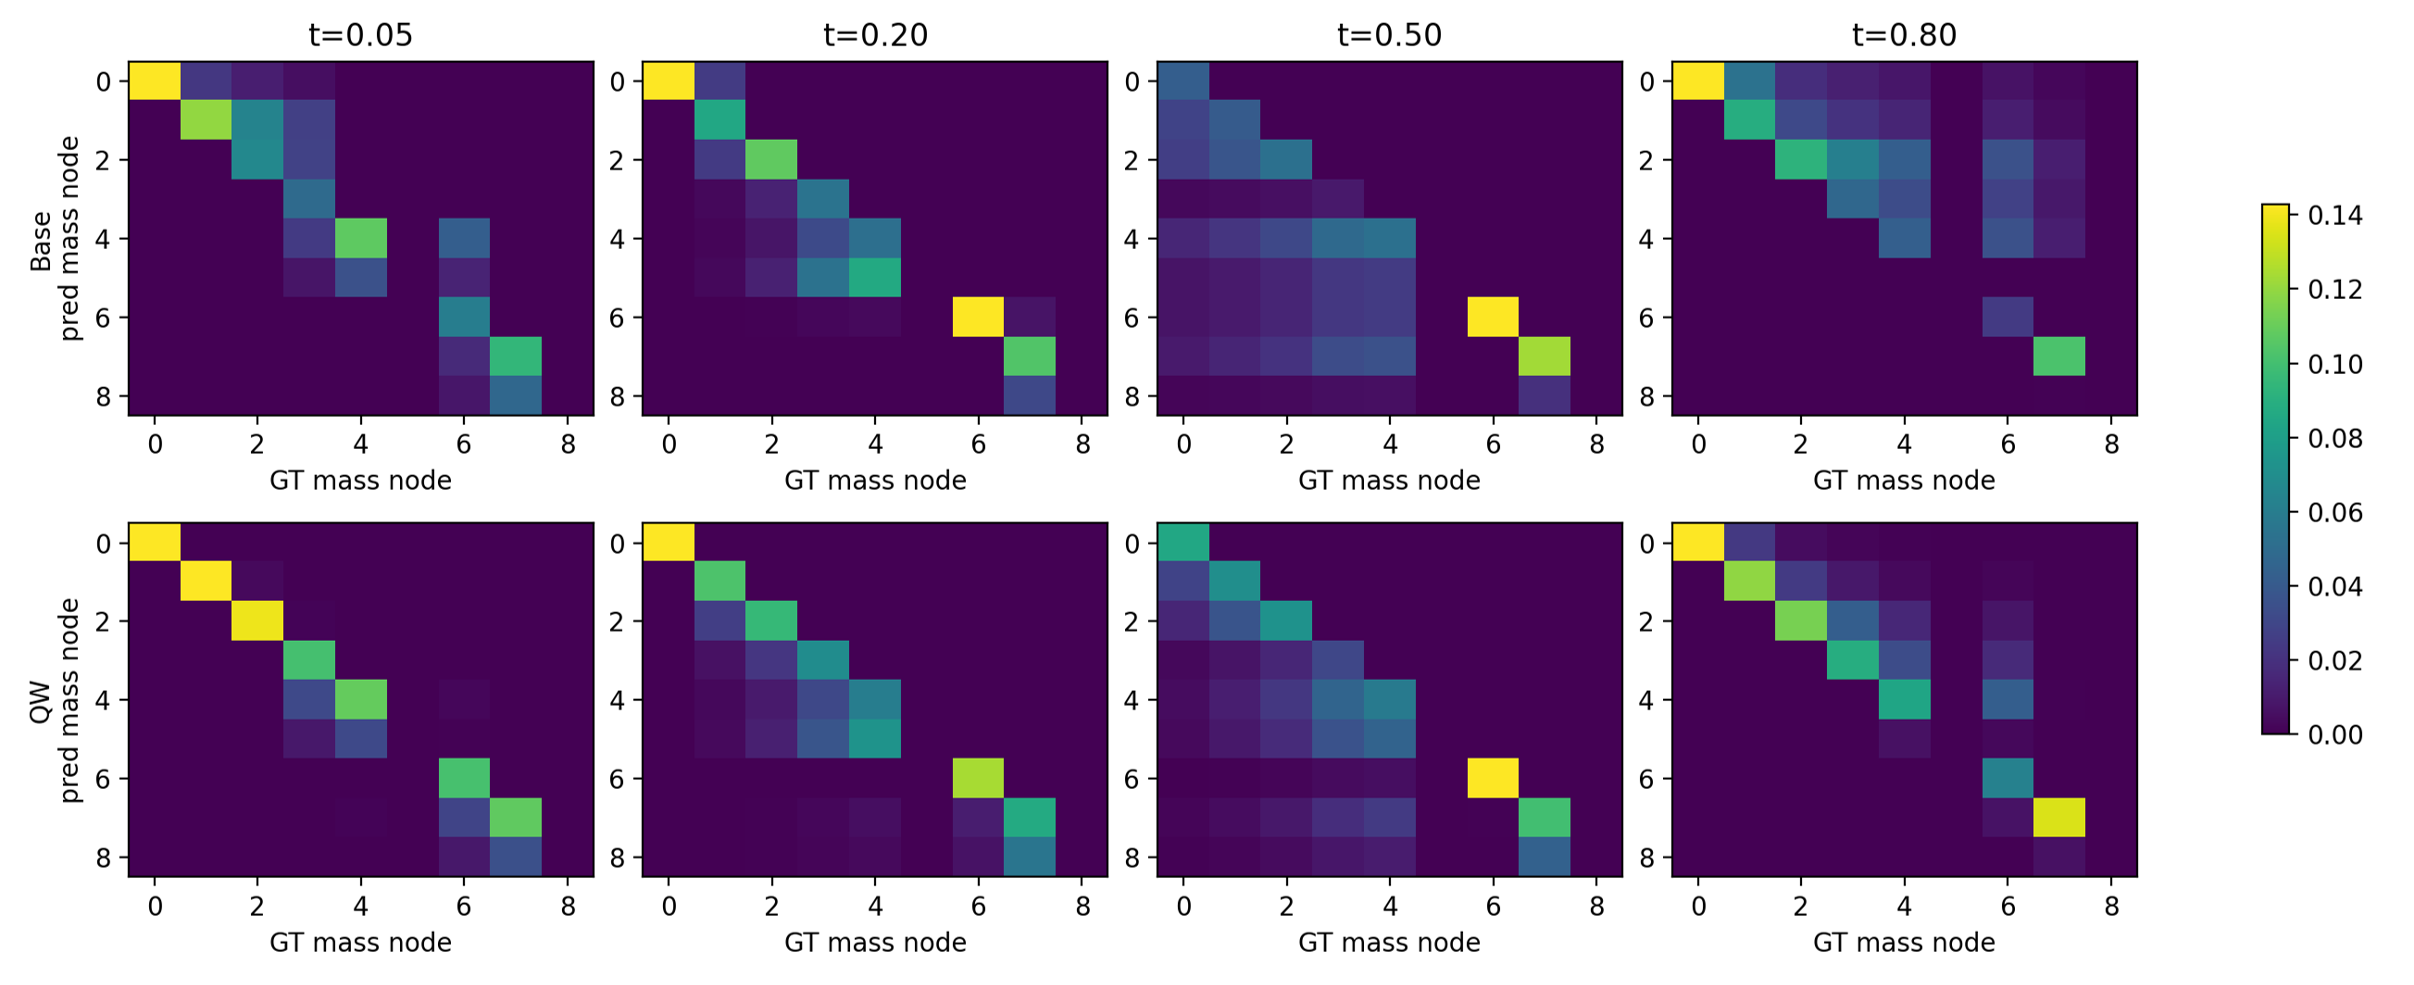
\includegraphics[width=.95\linewidth]{probing_ot_coupling.png}
    \caption{Sinkhorn coupling $P$ between the predicted node-type marginals and the ground truth under the shortest-path (geodesic) cost, probed at $t\in\{0.05,0.2,0.5,0.8\}$ on QM9 dataset.}
    \label{fig:ot-coupling-qm9}
\end{figure}
% \vspace{-3em}

\begin{figure}
    \centering
    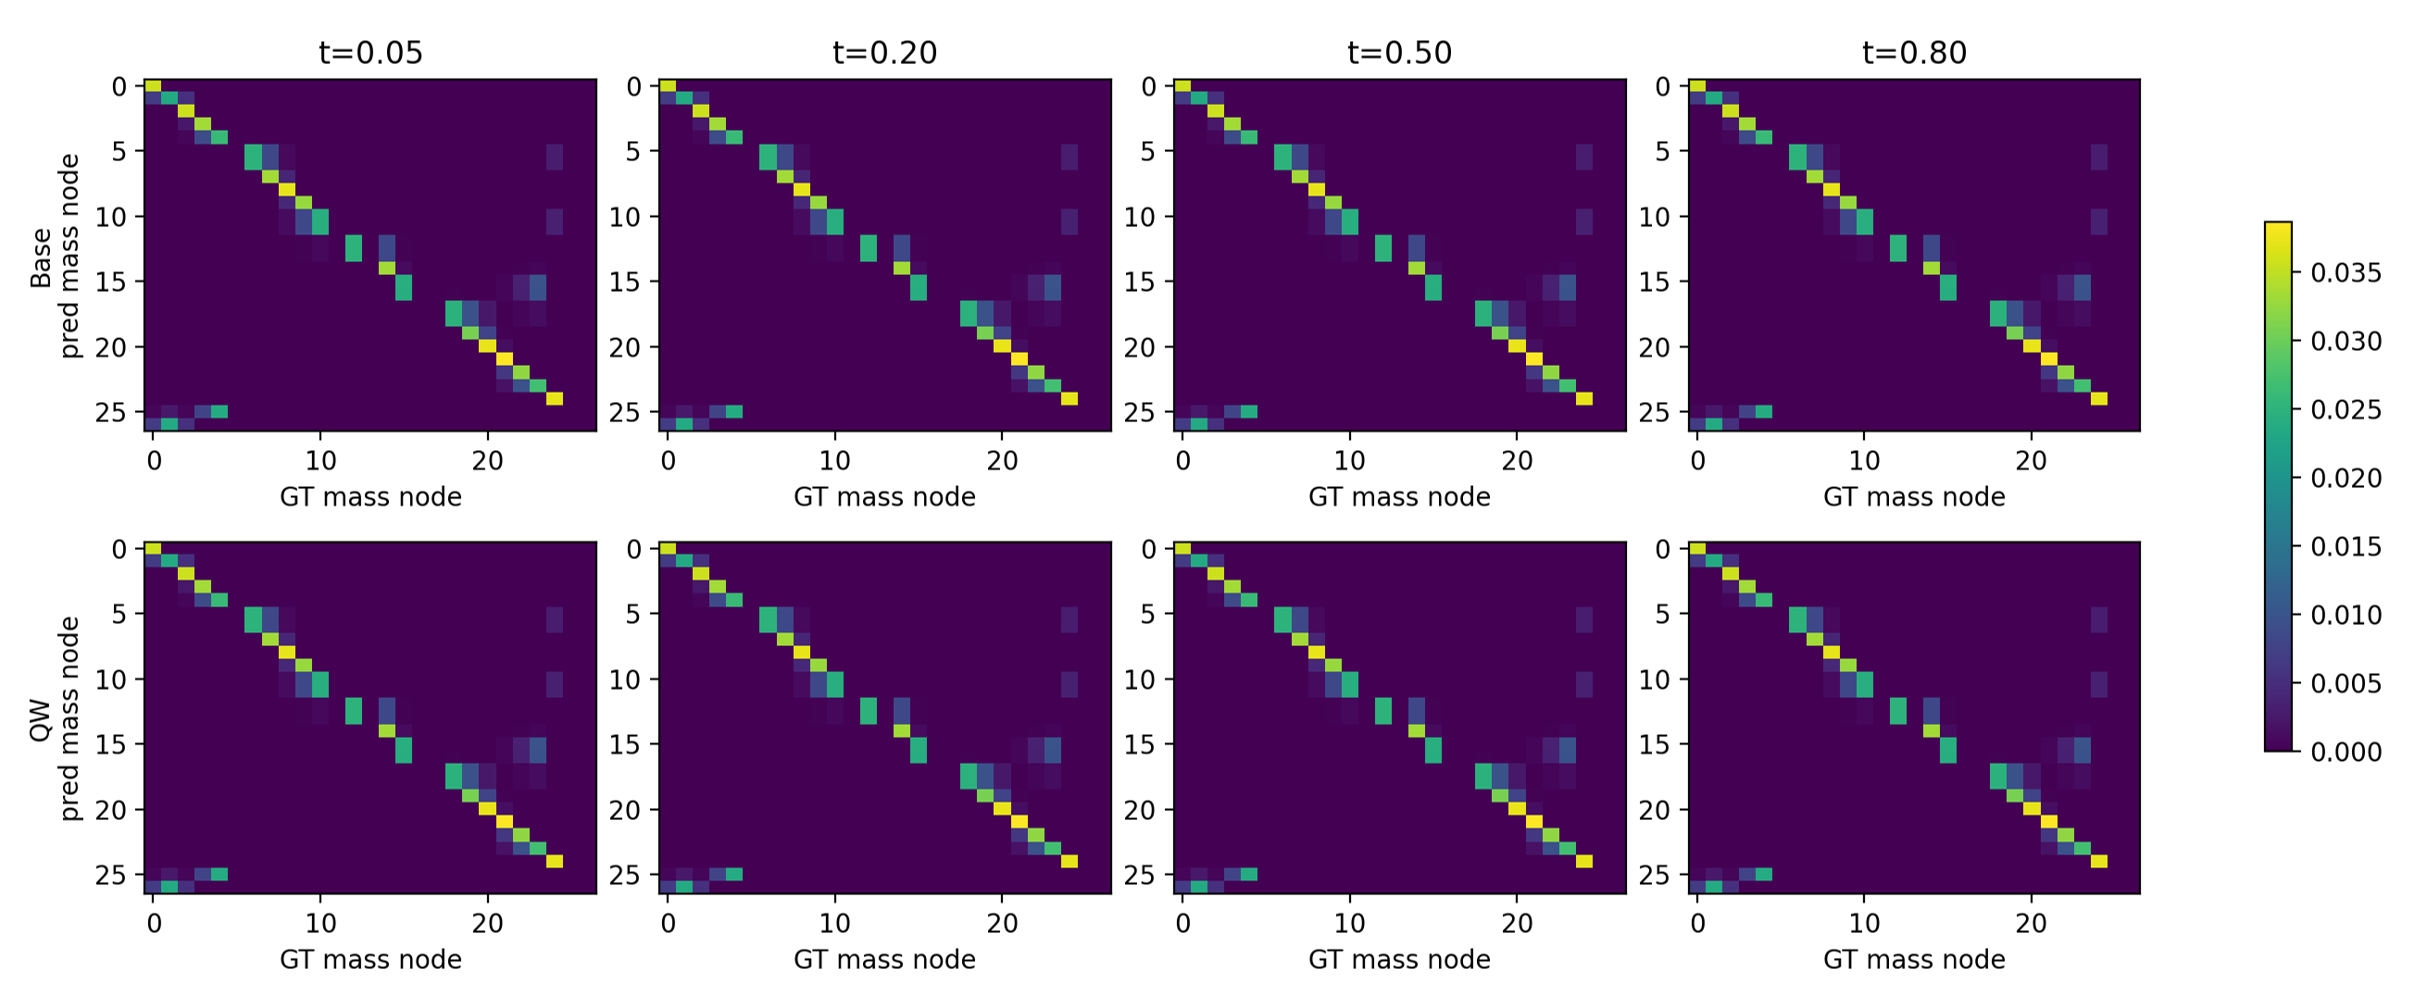
\includegraphics[width=.95\linewidth]{probing_ot_coupling_2.png}
    \caption{Sinkhorn coupling $P$ between the predicted node-type marginals and the ground truth under the shortest-path (geodesic) cost, probed at $t\in\{0.05,0.2,0.5,0.8\}$ on ZINC250k dataset.}
    \label{fig:ot-coupling-zinc250k}
\end{figure}
% \vspace{-3em}


% ---------------- Probing table ----------------
\begin{table}[t]
\centering
\caption{Probing statistics under shortest-path cost at $t\in\{0.05,0.2,0.5,0.8\}$ (Base vs.\ QW). QW reduces transport cost and increases local transport mass, indicating more geodesically local corrections.}
% \scriptsize
% \setlength\tabcolsep{3pt}
\renewcommand\arraystretch{1.15}
\begin{tabular*}{\textwidth}{@{\extracolsep{\fill}}c|ccc|ccc|ccc|ccc@{\extracolsep{\fill}}}
\toprule
\multirow{2}{*}{$t$} &
\multicolumn{3}{c|}{cost\_avg$\downarrow$} &
\multicolumn{3}{c|}{localmass1$\uparrow$} &
\multicolumn{3}{c|}{localmass2$\uparrow$} &
\multicolumn{3}{c}{avg\_pX\_gt$\uparrow$} \\
\cmidrule(lr){2-4}\cmidrule(lr){5-7}\cmidrule(lr){8-10}\cmidrule(lr){11-13}
& Base & QW & Improve & Base & QW & Improve & Base & QW & Improve & Base & QW & Improve \\
\midrule
0.05 & 0.834 & 0.605 & \textbf{27.5\%} & 0.810 & 0.852 & \textbf{5.2\%} & 0.911 & 0.923 & \textbf{1.3\%} & 0.328 & 0.495 & \textbf{50.9\%} \\
0.20 & 0.815 & 0.767 & \textbf{5.9\%}  & 0.800 & 0.813 & \textbf{1.6\%} & 0.901 & 0.911 & \textbf{1.1\%} & 0.347 & 0.602 & \textbf{73.5\%} \\
0.50 & 1.454 & 1.149 & \textbf{21.0\%} & 0.612 & 0.698 & \textbf{14.1\%} & 0.755 & 0.826 & \textbf{9.4\%} & 0.422 & 0.581 & \textbf{37.7\%} \\
0.80 & 0.800 & 0.344 & \textbf{57.0\%} & 0.761 & 0.913 & \textbf{20.0\%} & 0.913 & 0.987 & \textbf{8.1\%} & 0.552 & 0.707 & \textbf{28.1\%} \\
\hline
\end{tabular*}
\label{tab:probing_short}
\end{table}

% % ---------------- Sampling table ----------------
% \begin{table}[t]
% \centering
% \scriptsize
% \setlength\tabcolsep{3pt}
% \renewcommand\arraystretch{1.15}
% \begin{tabular}{c|ccc|ccc|ccc}
% \toprule
% \multirow{2}{*}{$t$} &
% \multicolumn{3}{c|}{entropy\_edge$\downarrow$} &
% \multicolumn{3}{c|}{entropy\_node$\downarrow$} &
% \multicolumn{3}{c}{pX\_max$\uparrow$} \\
% \cmidrule(lr){2-4}\cmidrule(lr){5-7}\cmidrule(lr){8-10}
% & Base & QW & Improve & Base & QW & Improve & Base & QW & Improve \\
% \midrule
% 0.05 & 0.974 & 0.947 & 2.8\%  & 0.809 & 0.918 & -13.5\% & 0.695 & 0.651 & -6.2\% \\
% 0.20 & 1.006 & 0.901 & 10.4\% & 0.509 & 0.947 & -86.1\% & 0.840 & 0.666 & -20.7\% \\
% 0.50 & 1.046 & 0.740 & 29.3\% & 0.598 & 1.175 & -96.4\% & 0.756 & 0.523 & -30.8\% \\
% 0.80 & 0.838 & 0.509 & 39.2\% & 0.381 & 1.029 & -170.2\%& 0.842 & 0.546 & -35.2\% \\
% \hline
% \end{tabular}
% \caption{Sampling-trajectory statistics at aligned time points. QW accelerates edge stabilization in this run (lower edge entropy), while node confidence can become more conservative.}
% \label{tab:sampling_short}
% \end{table}

\subsection{Interpretability Analysis}
\label{app:interpretability}

QW regularization is intended to encourage topology-consistent (geodesically local) corrections. To make this effect observable beyond final metrics, we report controlled probing at fixed noise levels $t$. We evaluate four representative noise levels $t\in\{0.05,0.2,0.5,0.8\}$.

For probing, we quantify locality via Sinkhorn-OT diagnostics under shortest-path cost: transport cost \texttt{cost\_avg}$\downarrow$ and local-mass ratios within 1/2 hops \texttt{localmass1/2}$\uparrow$, together with a correctness proxy \texttt{avg\_pX\_gt}$\uparrow$.
Improve is relative improvement: for $\downarrow$, $(\text{Base}-\text{QW})/\text{Base}$; for $\uparrow$, $(\text{QW}-\text{Base})/\text{Base}$.

Across noise levels, probing verifies the intended mechanism: QW promotes geodesically local corrections (lower $\texttt{cost\_avg}$, higher $\texttt{localmass1/2}$).

The coupling matrix $P$ transports the predicted node-type mass to the ground-truth mass with graph geodesic distance as the unit cost.
Mass concentrated near small distances indicates that correcting node-type distributions primarily involves local adjustments on the graph, whereas diffuse off-diagonal mass implies long-range relocation.
As shown in Figures~\ref{fig:ot-coupling-qm9} and~\ref{fig:ot-coupling-zinc250k}, QW produces a noticeably more localized transport plan than the Base model at the same noise level, consistent with the reduced \texttt{cost\_avg} and increased local-mass ratios in Table~\ref{tab:probing_short}.


\section{Visualization of Generated Molecular Graphs}
\label{app:vis}

We demonstrate some randomly selected molecular graphs generated by TopBF on both QM9 and ZINC250k datasets in Figures.~\ref{fig:samples_q} and~\ref{fig:samples_z}.

\begin{figure*}[!htbp]
    \centering
    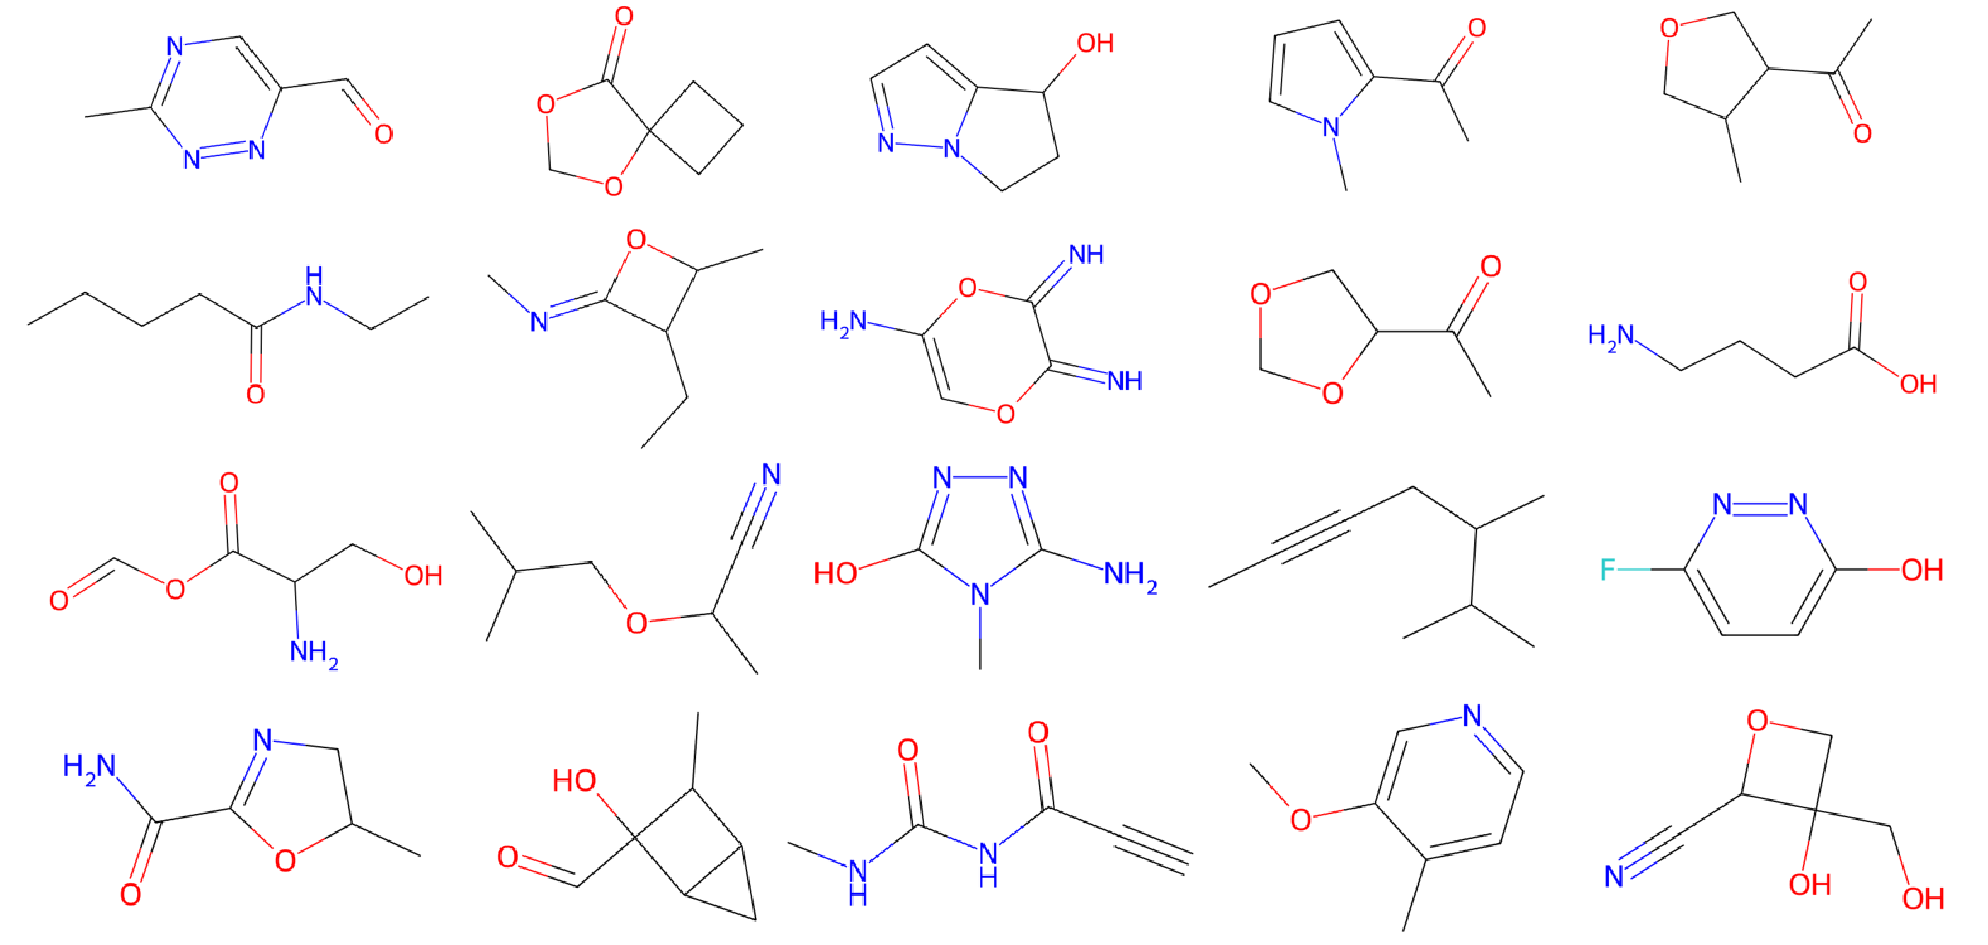
\includegraphics[width=0.95\linewidth]{samples_q.pdf}
    \caption{Molecular graphs generated by TopBF on QM9 dataset.}
    \label{fig:samples_q}
\end{figure*}

\begin{figure*}[!htbp]
    \centering
    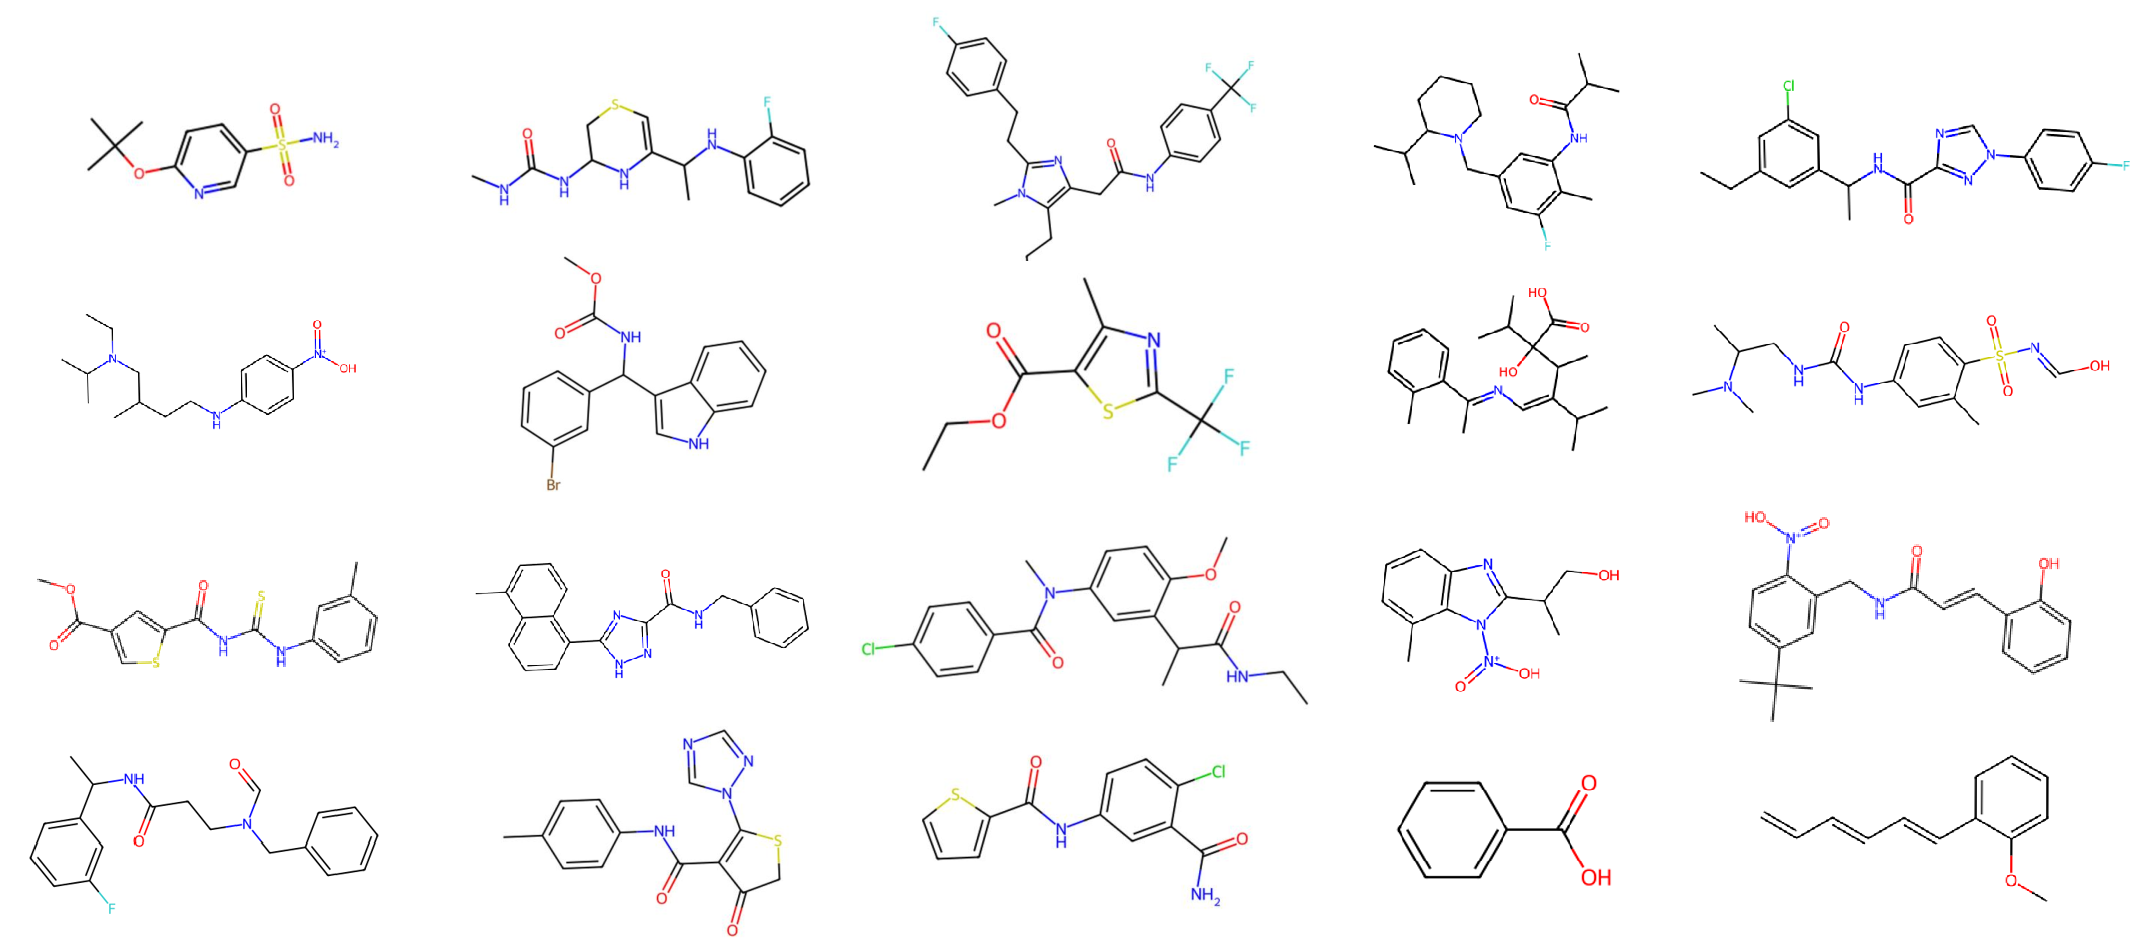
\includegraphics[width=0.95\linewidth]{samples_z.pdf}
    \caption{Molecular graphs generated by TopBF on ZINC250k dataset.}
    \label{fig:samples_z}
\end{figure*}


\section{Pseudocode for TopBF}
\label{app:pseudocode}

Pseudocode for essential functions in TopBF and continuous-time loss $\mathcal{L}_{\infty}$ are presented in Algorithms~\ref{alg:funtions} and~\ref{alg:train}, while sampling procedure is provided in Algorithm~\ref{alg:sample}, wherein $\text{NEAREST\_CENTER}$ compares the inputs to the nearest centers. 
% During sampling, TopBF generates new molecular graphs by reversing the Bayesian flow, starting from a simple prior over parameters and iteratively refining them towards plausible molecules over $n$ time steps. Algorithm~\ref{alg:sample} illustrates the sampling procedure, wherein $\text{NEAREST\_CENTER}$ compares the inputs to the nearest centers.

% =========================================================
\clearpage
\begin{multicols}{2} % 局部开启双栏

\begin{algorithm}[H]
\caption{Functions for TopBF}
\label{alg:funtions}
\begin{algorithmic}

\State \textbf{function} \textsc{CDF}$(\mu, \sigma, x)$
    \State $F(x) \gets \dfrac{1}{2}\left[1 + \mathrm{erf}\bigl(\dfrac{x-\mu}{\sqrt{2}\sigma}\bigr)\right]$
    \If{$x \le -1$}
        \State $H(x) \gets 0$
    \ElsIf{$x \ge 1$}
        \State $H(x) \gets 1$
    \Else
        \State $H(x) \gets F(x)$
    \EndIf
    \State \textbf{return} $H(x)$
\State \textbf{end function}
% \vspace{0.3em}

\State \textbf{function} \text{PRED}$(\mathbf{\mu} \in \mathbb{R}^{D\times K},\, t \in [0,1],\, K \in \mathbb{N},\, \gamma(t) \in \mathbb{R}^+,\, t_{\min} \in \mathbb{R}^+)$
    \State \# $t_{\min}$ is set to $0.0001$ by default
    \If{$t < t_{\min}$}
        \State $\hat{\mu} \gets 0,\,\, \hat{\sigma} \gets 1$
    \Else
        \State $\boldsymbol{\mu}_\epsilon, \ln \boldsymbol{\sigma}_\epsilon \gets \Psi(\boldsymbol{\theta}_t, \mathbf{c}, t)$
        \State $\hat{\boldsymbol{\mu}} \gets \frac{\boldsymbol{\mu}}{\gamma(t)} - \sqrt{\frac{1-\gamma(t)}{\gamma(t)}}\boldsymbol{\mu}_\epsilon$
        \State $\hat{\boldsymbol{\sigma}} \gets
            \sqrt{\frac{1-\gamma(t)}{\gamma(t)}}\text{exp}(\ln\boldsymbol{\sigma}_\epsilon)$
    \EndIf

    \For{$d = 1,\dots,D$}
        \For{each $k \in K$}
            \State $p_O^{(d)}(k\,|\,\theta) \gets
                \text{CDF}(\hat{\mu}^{(d)},\hat{\sigma}^{(d)},k_r)
                - \text{CDF}(\hat{\mu}^{(d)},\hat{\sigma}^{(d)},k_l)$
        \EndFor
    \EndFor

    \State \textbf{return} $p_O(\cdot \mid \boldsymbol{\theta}_t)$
\State \textbf{end function}

\end{algorithmic}
\end{algorithm}

% =========================================================

\begin{algorithm}[H]
    \caption{Training Algorithm} 
    \begin{algorithmic}
        \Require $\sigma_{1}\in \mathbb{R}^+, K \in \mathbb{N}$
        \State \textbf{Input:} parameterized continuous graph $\mathbf{G}$
        \State $t \sim \mathcal{U}(0, 1)$
        \State $\gamma \gets 1 - \sigma_{1}^{2t}$
        \State $\mathbf{\mu} \sim \mathcal{N}(\gamma(t), \gamma(t)(1-\gamma(t))\boldsymbol{I})$
        \State $p_{O}(\cdot \mid \boldsymbol{\theta}_t) \gets \text{PRED}(\boldsymbol{\mu}, t, K, \gamma(t))$
        \State $\hat{\mathbf{k}}_{c}(\boldsymbol{\theta}_t, t) \gets \text{NEAREST\_CENTER}\big(p_O(\cdot \mid \boldsymbol{\theta}_t)\big)$
        \State $\mathcal{L}_{\infty}(\mathbf{G}) \gets -\ln \sigma_{1}\sigma_{1}^{-2t}\|\mathbf{G}-\hat{\mathbf{k}}_{c}(\boldsymbol{\theta}_t, t)\|_2^2$ 
        \Return $\mathcal{L}_{\infty}(\mathbf{G})$
    \end{algorithmic} 
    \label{alg:train}
\end{algorithm}


% \begin{algorithm} 
%     \caption{Sampling Algorithm} 
%     \begin{algorithmic}
%         \Require $\sigma_{1}\in \mathbb{R}^+, \text{number of steps}\,\,n, K \in \mathbb{N}, \mathbf{c} \gets \text{None}$
%         \State $\boldsymbol{\mu} \gets \mathbf{0}, \,\,\rho \gets 1$
%         \For{$i=1\;\text{to}\;n$}
%         \State $t \gets \frac{i-1}{n}$
%         \State $\gamma(t) \gets 1-\sigma_{1}^{2t}$
%         \State $p_{O}(\cdot \mid \boldsymbol{\theta}_t) \gets \text{PRED}(\boldsymbol{\mu}_t, t, K, \gamma(t), \mathbf{c})$
%         \State $\alpha(t) \gets \sigma_{1}^{-2i/n}\big( 1 - \sigma_{1}^{2/n} \big)$
%         \State $\mathbf{Y} \sim \mathcal{N}(\mathbf{k}_{c}, \alpha(t)^{-1}\boldsymbol{I})$
%         \State $\boldsymbol{\mu}_{i} \gets \frac{\rho_{i-1} \boldsymbol{\mu}_{i-1} + \alpha(t) \mathbf{Y}}{\rho_{i-1} + \alpha(t)}$
%         \State $\rho_{i} \gets \rho_{i-1} + \alpha(t)$
%         \EndFor
%         \State $p_{O}(\cdot \mid \boldsymbol{\theta}_1) \gets \text{PRED}(\boldsymbol{\mu}, 1, K, 1-\sigma_{1}^2, \mathbf{c})$
%         \State $k'_{c}(\boldsymbol{\theta}_1, 1) \gets \text{NEAREST\_CENTER}(\boldsymbol{\theta}_1, 1)$
%         \Return $k'_{c}(\boldsymbol{\theta}_1, 1)$
%     \end{algorithmic} 
%     \label{alg:sample}
% \end{algorithm}

\begin{algorithm}[H]
    \caption{Sampling Algorithm} 
    \begin{algorithmic}
        \Require $\sigma_{1}\in \mathbb{R}^+$, number of steps $n$, $K \in \mathbb{N}$, optional $\mathbf{z}^\star$, $\lambda \geq 0$
        \State $\boldsymbol{\mu}_0 \gets \mathbf{0}, \,\,\rho_0 \gets 1$
        \For{$i=1\;\textbf{to}\;n$}
            \State $t \gets \frac{i-1}{n}$
            \State $\gamma(t) \gets 1-\sigma_{1}^{2t}$
            \State $\boldsymbol{\theta}_t \gets (\boldsymbol{\mu}_{i-1}, \rho_{i-1})$
            \If{$\mathbf{z}^\star$ is not None \textbf{and} $\lambda > 0$}
                % \State $\hat{\mathbf{G}}_t \gets \text{DECODE\_MEAN}(\boldsymbol{\theta}_t, t)$
                % \State $\hat{\mathbf{z}}_t \gets R_\varphi(\hat{\mathbf{G}}_t, t)$
                \State $\hat{\mathbf{z}}_t \gets R_\varphi(\boldsymbol{\theta}_t, t)$
                \State $\mathcal{L}_{\text{prop}} \gets \|\hat{\mathbf{z}}_t - \mathbf{z}^\star\|_2^2$
                \State $\boldsymbol{\mu}_{i-1} \gets \boldsymbol{\mu}_{i-1}
                    - \lambda \nabla_{\boldsymbol{\mu}_{i-1}} \mathcal{L}_{\text{prop}}$
                \State $\boldsymbol{\theta}_t \gets (\boldsymbol{\mu}_{i-1}, \rho_{i-1})$
            \EndIf
            \State $p_{O}(\cdot \mid \boldsymbol{\theta}_t) \gets \text{PRED}(\boldsymbol{\mu}_{i-1}, t, K, \gamma(t))$
            \State $\alpha(t) \gets \sigma_{1}^{-2i/n}\big( 1 - \sigma_{1}^{2/n} \big)$
            \State $\mathbf{k}_{c}(\boldsymbol{\theta}_t, t) \gets \text{NEAREST\_CENTER}\big(p_O(\cdot \mid \boldsymbol{\theta}_t)\big)$
            \State $\mathbf{Y} \sim \mathcal{N}(\mathbf{k}_{c}(\boldsymbol{\theta}_t, t), \alpha(t)^{-1}\boldsymbol{I})$
            \State $\boldsymbol{\mu}_{i} \gets \dfrac{\rho_{i-1} \boldsymbol{\mu}_{i-1} + \alpha(t) \mathbf{Y}}{\rho_{i-1} + \alpha(t)}$
            \State $\rho_{i} \gets \rho_{i-1} + \alpha(t)$
        \EndFor
        \State $p_{O}(\cdot \mid \boldsymbol{\theta}_1) \gets \text{PRED}(\boldsymbol{\mu}_{n}, 1, K, 1-\sigma_{1}^2)$
        \State $k'_{c}(\boldsymbol{\theta}_1, 1) \gets \text{NEAREST\_CENTER}\big(p_O(\cdot \mid \boldsymbol{\theta}_1)\big)$
        \Return $k'_{c}(\boldsymbol{\theta}_1, 1)$
    \end{algorithmic} 
    \label{alg:sample}
\end{algorithm}
\end{multicols}

% \begin{figure*} % 考虑放到附录，这样可以多放一些分子图
%     \centering
%     \includegraphics[width=0.95\linewidth]{samples.pdf}
%     \caption{Samples generated by TopBF on ZINC250k and QM9 datasets.}
%     \label{fig:samples}
% \end{figure*}


\bibliographystyle{IEEEtran}
\bibliography{reference}

\end{document}
